\label{appendix_a}

One of the principle aims of this paper was to recreate and extend figures from \citet{McDougall1987}. They are reproduced below for completeness. 

\begin{figure}[htbp]
    \centering
    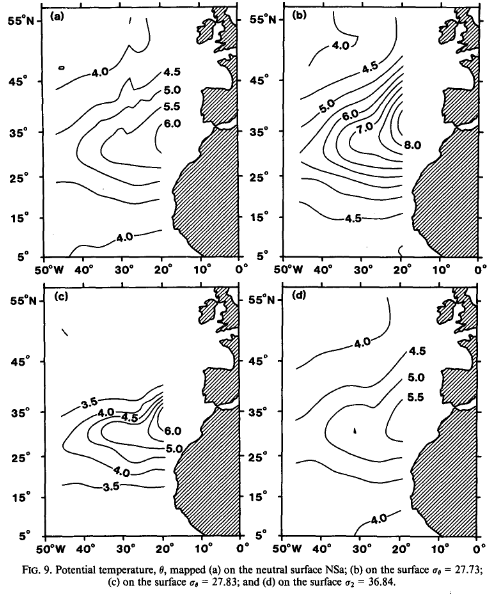
\includegraphics{mcdougall_fig_9}
    \caption{Potential temperature, $\theta$, mapped onto (a) neutral surface ``Nsa", referred to as $\gamma_n = 27.87$ in this paper (b) $\sigma_0 = 27.73$ (c) $\sigma_0 = 27.83$ and (d) $\sigma_0 = 36.84$ \citep{McDougall1987}. Also shown in section \ref{subsubsection:spreadmethodatlanticocean}}
    \label{fig:appendix_mcdougall_theta_spread}
\end{figure}

\begin{figure}[htbp]
    \centering
    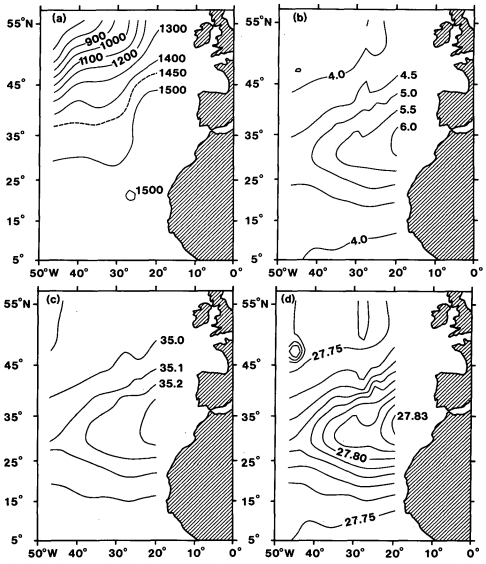
\includegraphics{plots/mc_dougall_fig_6.PNG}
    \caption{Maps of (a) pressure (b) $\theta$ (c) $S$ and (d) $\sigma0$ on the neutral surface ``Nsa" or $\gamma_n = 27.87$ \citep{McDougall1987}}
    \label{fig:appendix_mcdougall_neutral_surface_maps}
\end{figure}